\documentclass{beamer}

% \usepackage{beamerthemesplit} // Activate for custom appearance

\title{Two Efficiency Wage Models\\\large Perspectives on Economics TA Sessions}
\author{Qing Zhang}
\institute{Columbia University}
\date{\today}

\begin{document}

\frame{\titlepage}

\frame
{
  \frametitle{Today}

  \begin{itemize}
  \item How do we explain unemployment? Why does labor market not clear?    
  \item Efficiency wage theories: it pays firms to pay workers higher than the market-clearing wage. 
  \item Today we are going to talk about two of these models.
  \item Akerlof and Yellen, The Fair Wage-Effort Hypothesis and Unemployment:\\ Worker effort increases with wage paid.
  \item Shapiro and Stiglitz, Equilibrium Unemployment as a Worker Discipline Device:\\ Unemployment is necessary to prevent workers from shirking. 
  \end{itemize}
}

%\frame{
%\frametitle{Overview}
%\begin{itemize}
%\item The threat of firing is not the only way to discipline workers. For example, could make shirking workers who are caught pay a penalty, or not go through pay rises. But this could give firms an incentive to claim that workers have shirked when they have not. 
%\item Therefore, this paper may better be viewed as providing one possible explanation for unemployment - a result of imperfect monitoring in certain contexts.  
%\item The model was widely used in both labor economics and macroeconomics. 
%\end{itemize}
%}

\frame{
\frametitle{Akerlof and Yellen: Simplest Model}
\begin{itemize}
\item Worker effort is given by 
\[e = \text{min} (w/w^*, 1)\]
where $w^*$ is the fair wage. 
\item Production function of the firm
\[Q = \alpha eL\]
\item $eL$ is effective labor. This setup implies that the cost of one unit of effective labor is always $w^*$ when $w\leq w^*$. 
\end{itemize}
}

\frame{
\frametitle{Equilibrium}
\begin{itemize}
\item There are two cases. 
\item If $\alpha < w^*$, marginal product of effective labor ($\alpha$) is always smaller than marginal cost of effective labor ($w^*$). It is not profitable for firms to operate. Therefore unemployment rate is one. 
\item Generate equilibrium unemployment in a very simple model. 
\item If $\alpha > w^*$, firms want to hire infinite labor. In equilibrium, unemployment is zero, and equilibrium wage is bid up to $\alpha$. 
\end{itemize}
}


\frame{
\frametitle{Shapiro and Stiglitz}
\begin{itemize}
\item Firm cannot observe workers' effort, and can only caught shirking workers randomly. Need to impose a penalty on shirkers. 
\item The penalty here is unemployment. Workers are fired if caught shirking. 
\item They discuss other possible penalties, such as having workers post a bond and forfeit the bond if caught shirking. They argue that these other approaches open up possibilities for dishonest behavior on the part of the employer. 
\item In this world, unemployment becomes necessary for providing incentives. Full employment means no penalty for shirking because workers who are fired can immediately find a new job. 
\end{itemize}
}

\frame{
\frametitle{Worker Effort Decision}
\begin{itemize}
\item Workers make a single decision: to shirk or not, trading off leisure with possibility of being fired. 
\item This seems to be a dynamic programming problem, but not really. We assume the environment does not change over time. Then the decision will be the same every period. 
\item Worker utility per period $U = w-e$. Effort can be either 0 or some fixed level. 
\item Probability $q$ per period of being caught when shirking. Probability $b$ of exogenous job separation per period. 
\item Define $V_E^S$ as the expected lifetime utility of an employed shirker, $V_E^N$ as the expected lifetime utility of an employed non-shirker, $V_u$ as the expected lifetime utility of an unemployed worker. 

\end{itemize}

}

\frame{
\frametitle{Worker Effort Decision}
\begin{itemize}
\item For a short period $[0,t]$, $V_E^S = wt + (1-rt)[(b+q)tV_u + (1-(b+q)t)V_E^S]$
\item Solving for $V_E^S$ and taking $t \to 0$, we have $V_E^S = \frac{w + (b+q)V_u}{r+b+q}$.
\item Following the same steps, $V_E^N = \frac{w - e + bV_u}{r+b}$.
\item Assume workers are risk neutral. Then they will choose not to shirk if $V_E^N \geq V_E^S$. 
\item This is equivalent to 
\[w \geq \bar{w} + e + (a+b+r)e/q\]
No-shirking condition (NSC). $\bar{w}$ is per period unemployment benefit, $a$ is job finding rate. 
\end{itemize}

}

\frame{
\frametitle{Firms' Problem}
\begin{itemize}
\item Assume each firm has the same production function. 
\item Each firm chooses wage $w$ and unemployment benefit $\bar{w}$, and how much labor to hire. Firms are paying unemployment benefits because government is assumed away in this model. 
\item First, notice that firms will set $\bar{w}$ to the lowest level possible, since there are no benefits to the firm from paying unemployment benefits - a higher $\bar{w}$ necessitates a higher $w$, via the NSC.  
\item So workers are not insured. 
\end{itemize}
}

\frame{
\frametitle{Equilibrium}
\begin{itemize}
\item Equilibrium occurs when each firm, taking as given the wages and employment levels at other firms, finds it optimal to offer the ongoing wage. 
\item NSC:
\[w \geq \bar{w} + e + (a+b+r)e/q\]
\item Employed workers have higher utility than unemployed workers. The difference (in a single period) is $(a+b+r)e/q$. So the unemployed are involuntarily unemployed. They want to work at lower than the equilibrium wage, but firms won't lower wage because that would encourage incumbent workers to shirk. 
\item Flow into unemployment equals flow out of unemployment:
\[bL = a(N-L) \implies a=bL/(N-L)\]
\end{itemize}
}

\frame{
\frametitle{Equilibrium}
\begin{figure}
\centering
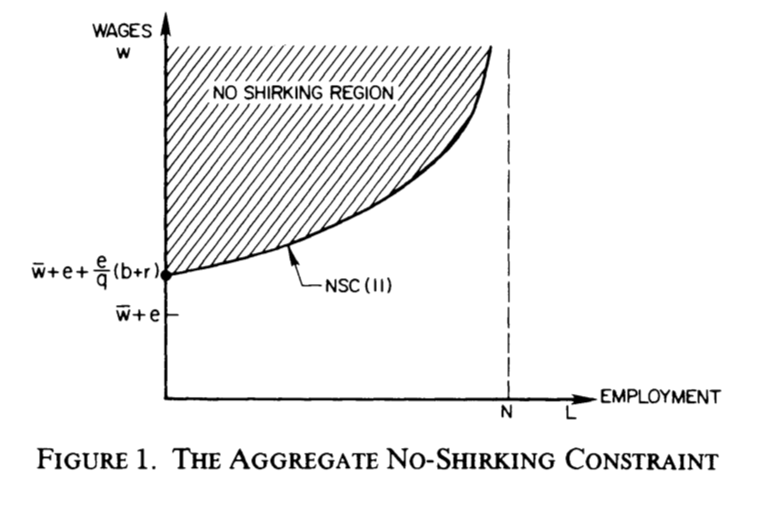
\includegraphics[width=0.8\textwidth]{f1}
\end{figure}
}

\frame{
\frametitle{Equilibrium}
\begin{figure}
\centering
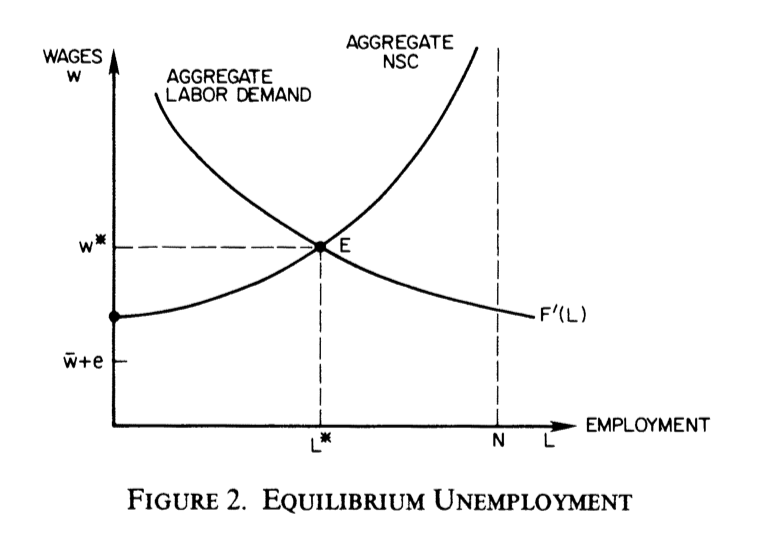
\includegraphics[width=0.6\textwidth]{f2}
\end{figure}
\begin{itemize}
\item Given that all other firms pay $w^*$, it is optimal for a firm to pay $w^*$.
\item If the firm pays lower than $w^*$, workers will shirk (in which case we assume the output is 0).
\item No need to pay higher than $w^*$, because the firm can hire as much labor as it wants at $w^*$ (labor market is competitive). 
\end{itemize}
}

\frame{
\frametitle{Discussion}
\begin{itemize}
\item When employers can select the monitoring intensity $q$ at a cost, they will choose too much monitoring (relative to efficiency), which leads to too much employment (under constant returns to scale technology). 
\item The idea is that a larger unemployment pool will increase the threat of unemployment and make workers less likely to shirk. When hiring workers, employers do not consider the externality of hiring through its effect on the unemployment pool. 
\item They could have chosen lower employment, and saved on monitoring (supervision) costs. 
\item If there are other costs associated with dismissal, such as search costs, moving expenses, loss of job-specific human capital, etc, the need for an efficiency wage will be dampened. 
\end{itemize}
}

\end{document}
